\newpage
\chapter{Desenvolvimento}
\label{ch:desenvolvimento}

% \par Este capítulo irá detalhar como as novas funcionalidades foram desenvolvidas para o framework Esfinge Gamification.

%\par Como o Esfinge Gamification é utilizado por outros desenvolvedores, o projeto \textbf{DrawableNNAPI}\footnote{O projeto está disponível em: https://gitlab.com/django-livre/DrawRestfulAPI} foi desenvolvido a fim de identificar possíveis melhorias e/ou novas funcionalidades que poderiam ser aplicadas no framework.

%\section{Método \textit{getAllAchievements}}
%\par Foi criado um método para recuperar todos as conquistas por tipo, como a próxima listagem irá exibir, este método recebe como parâmetro uma classe que estenda a classe abstrata \textit{Achievement}, portanto uma conquista, a partir deste parâmetro as conquistas serão recuperadas. A utilidade deste método é o auxilio na criação de rankings e/ou a comparações entre todos os usuários.

\par Explicar alguma historinha pra contextualizar


\section{Fluxo de funcionamento}
%talvez inserir proxy dinamico no capítulo 2
\par O framework possui o fluxo de funcionamento apresentado na Figura \ref{fig:fluxo-atual}. 

\begin{figure}[H]
    \centering
    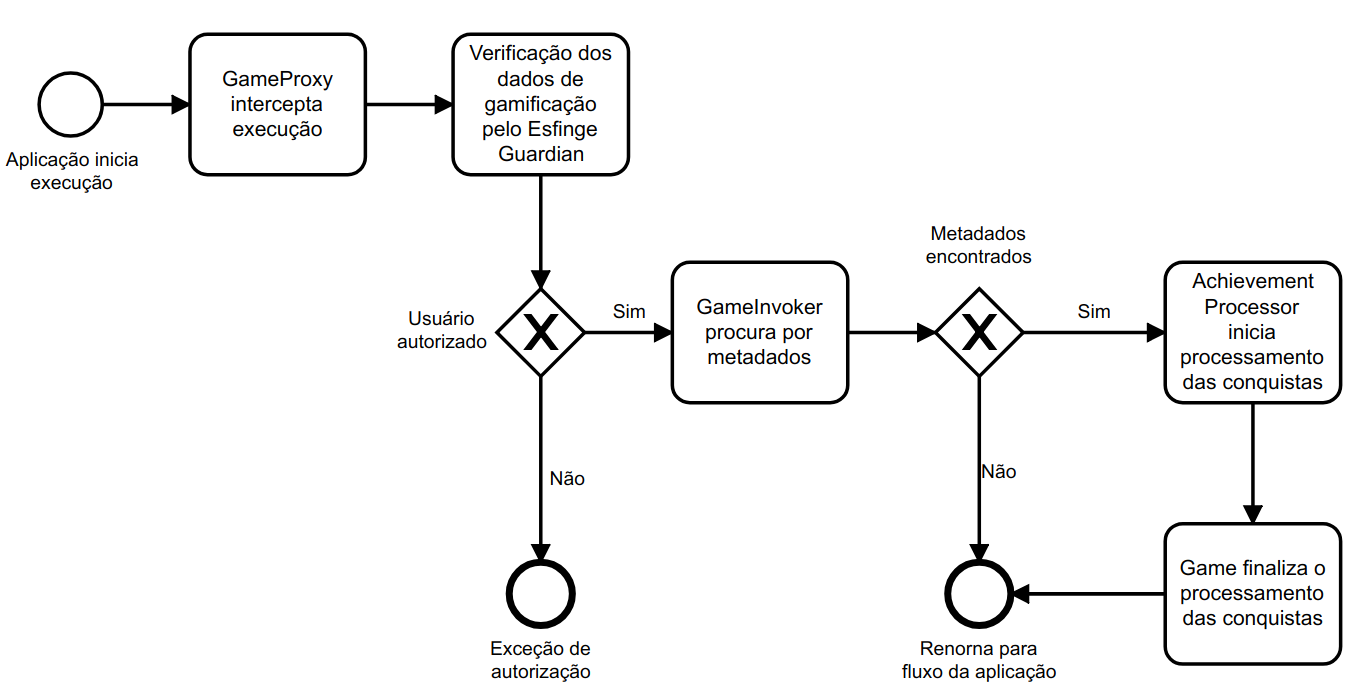
\includegraphics[scale=0.3]{src/imagens/cap3/fluxo-atual.png}
    \caption{Fluxo de funcionamento atual do Esfinge Gamification}
    \label{fig:fluxo-atual}
\end{figure}

Neste fluxo, aplicações em que o Esfinge Gamification foi configurado, são interceptadas via \textit{Proxy} Dinâmico e antes do fluxo de gamificação ser executado o \textit{Proxy} Dinâmico do Esfinge Guardian é invocado para que validações de autorização do usuário sejam realizadas. Na linha 14 da Figura \ref{fig:esfinge-proxy} um objeto que será interceptado pelo Esfinge Guardian é criado, e na linha 8 em que o método recebido pelo Proxy Dinâmico do Esfinge Gamification é invocado o objeto passado como parâmetro para a invocação é o Proxy Dinâmico do Esfinge Guardian, desta forma a responsabilidade de execução é passada para o Esfinge Guardian e as validações ocorrem.

\begin{figure}[H]
    \centering
    \begin{java}
public class GameProxy implements InvocationHandler {

    // Objetos omitidos

    private GameProxy(Object encapsulated) {
                this.encapsulated = encapsulated;
    	// tratativa de excecao omitida
    	this.guardedObject = AuthorizationContext.guardObject(encapsulated);
    	
    }

    public Object invoke(Object proxy, Method method, Object[] args) throws Throwable {
    	try {
        	Object returnValue = method.invoke(guardedObject, args);
        	GameInvoker gameInvoker = GameInvoker.getInstance();
        	gameInvoker.registerAchievment(encapsulated, method, args);
    
    	    return returnValue;
    	} catch (InvocationTargetException e) {
    	    throw e.getTargetException();
    	}
    }
    
    public static <T> T createProxy(T encapsulated) {
    	Object obj = Proxy.newProxyInstance(
                    encapsulated.getClass().getClassLoader(),
                    encapsulated.getClass().getInterfaces(), 
                    new GameProxy(encapsulated)
    	);
    
    	// validacao do Esfinge Metadata validator omitida
    	return (T) obj;
    }
}
    \end{java}
    \caption{Criação do \textit{proxy} dinâmico do Esfinge Gamification}
    \label{fig:esfinge-proxy}
    \fonte{Produção do autor}
\end{figure}


Após a validação o fluxo de execução é devolvido para o Esfinge Gamification, que procura por metadados e caso alguma implementação da interface \textit{Achievement Processor} for encontrada nos metadados esta é invocada para que os dados de gamificação sejam pré processados. Depois de pré processados os dados são enviados para a especialização escolhida da classe \textit{Game}. Por fim, quando os dados são processados o fluxo é devolvido para a aplicação.

\section{Visão geral}

\par Esta seção tem como objetivo explicar como o framework é usado do jeito mais básico possível, a Figura \ref{fig:hello-world-gamification} realiza a configuração do Esfinge Gamification em um ambiente em que notas podem ser atribuídas a usuários apenas por quem possuir o Ranking \textit{Avaliator} e o Level \textit{Master}. 


\begin{figure}[H]
    \centering
    \begin{java}
    public class AuthorizationSample {
    
	public static void main(String[] args) {

		User user = new User();
		user.setClassroom("C12019");
		user.setRa("C1A252019");
		
		// Metodo de gerencia de conquistas (armazenamento de memoria)
		Game game = new GameMemoryStorage();

		// Configuracao do Esfinge Gamification
		GameInvoker.getInstance().setGame(game);
		UserStorage.setUserID(user.getRa());

		// Cria um objeto para ser monitorado pelo Esfinge Guardian
		User guardedUser = AuthorizationContext.guardObject(user);

		guardedUser.addNote(10.0);

	}
}
    \end{java}
    \caption{Configuração e utilização do \textit{framework}}
    \label{fig:hello-world-gamification}
    \fonte{Produção do autor}
\end{figure}

Neste exemplo o usuário atual tenta alterar seus pontos e recebe a exceção \textit{"Unauthorized Access"} do pacote \textit{org.esfinge.guardian.exception.AuthorizationException} devido a falta do Ranking necessário, a Figura \ref{fig:execao-configuracao} exibe a configuração realizada na classe \textit{User} para que a autorização seja monitorada pelo Esfinge Guardian.

\begin{figure}[H]
    \centering
    \begin{java}
    public class User {

	private String classroom;
	private String ra;
	private List<Double> notes;

	public User(String classroom, String ra, List<Double> notes) {
		super();
		this.classroom = classroom;
		this.ra = ra;
		this.notes = notes;
	}
    
    // Anotacao de configuracao
	@AllowRankingAndLevel(achievementName = "Avaliator", level = "Master")
	public void addNote(Double note) {
		List<Double> notes = this.getNotes();
		Objects.requireNonNull(notes, "Notes can't be null");
		notes.add(note);
	}
	
	// Getters and setters omitidos
	
	}
    \end{java}
    \caption{Configuração de segurança da classe \textit{User}}
    \label{fig:execao-configuracao}
    \fonte{Produção do autor}
\end{figure}

\section{Funcionalidades}

\par Para o controle de conquistas as anotações da Tabela \ref{tab:autorizacoes} foram criadas.

\begin{longtable}{|l|m{10cm}|}
\hline
Anotação & Comportamento \\ \hline
\endfirsthead
\endhead
\begin{tabular}[c]{@{}l@{}}
@AllowPointGreaterThan, \\ @AllowPointLessOrEqualsThan, \\ @DenyPointLessOrEqualsThan, \\ @DenyPointGreaterThan
\end{tabular} & Estas anotações verificam se os pontos respeitam as restrições de maior ou menor igual a uma determinada quantidade de pontos definida na anotação para que a autorização seja permitida ou não. \\ \hline
\begin{tabular}[c]{@{}l@{}}
@AllowRanking, \\
@AllowLevel, \\ 
@AllowRankingAndLevel, \\
@AllowRankingOrLevel, \\ 
@DenyLevel, \\
@DenyRanking, \\ 
@DenyRankingAndLevel, \\
@DenyRankingOrLevel
\end{tabular} & As anotações de ranking possuem a mesma lógica das anteriores, porém, visando os recursos do ranking, permitindo e não permitindo o acesso a recursos com as restrições de ranking e level. \\ \hline
@AllowTrophy, @DenyTrophy & Estas anotações verificam o acesso de usuários a recursos protegidos com a restrição de troféu, isto é, quando algum usuário possuir o troféu conseguirá ou não acessar o recurso. \\ \hline
@AllowReward, @DenyReward & Estas anotações verificam o acesso de usuários a recursos protegidos com a restrição de recompensa, isto é, quando algum usuário possuir o recompensa conseguirá ou não acessar o recurso. \\ \hline
\caption{Anotações de autorização}
\fonte{Produção do autor}
\label{tab:autorizacoes}\\
\end{longtable}
